% ----------------------------------------------------------
\chapter{Metodologia
}\label{cap:desenvolvimento}
% ----------------------------------------------------------
\section{Interface gráfica}

A interface gráfica publicada no navegador foi elaborada utilizando CSS, JavaScript e HTML. 

\section{Representação tridimensional}

As representações tridimensionais moleculares foram feitas com Three.js, uma biblioteca que usa WebGL para desenhar (na realidade, renderizar) objetos 3D de maneira facilitada. 

\section{Método de Hueckel Estendido}

O \gls{HMO} foi inicialmente proposto por Erich Hueckel em 1930 \autocite{Hckel1931} como uma alternativa para calcular orbitais moleculares como combinações lineares de orbitais atômicos\autocite{Coulson1978-ot}. Tal teoria prediz os orbitais moleculares de elétrons $\pi$ em moléculas com estrutura eletrônica deslocalizada., tal como o etileno, benzeno, butadieno e piridina. Isso nos fornece uma base teórica para fundamentar a regra de Hueckel, responsável por enunciar que moléculas cíclicas, planares ou espécies químicas iônicas com $4n + 2$ elétrons $\pi$ são aromáticos.

Esse modelo baseia-se no fato de que a interação entre dois orbitais atômicos (sobreposição) produz um orbital molecular ligante mais estável (energia mais baixa), e um orbital molecular antiligante, menos estável do que aqueles que o geraram. Dessa forma, o número de orbitais moleculares novos é igual ao número de orbitais atômicos envolvidos (a combinação linear). A estabilidade relativa ou as energias dos orbitais moleculares em um polieno completamente conjugado, cíclico, planar pode ser predita pela teoria de Hueckel. Tomando o benzeno como exemplo, é possível ilustrar, através de um círculo de Frost (\autoref{fig:M1}), os níveis de energia dos seus orbitais moleculares de fronteira.

\begin{figure}[htb]
	\caption{\label{fig:M1} Círculo de Frost para o benzeno.}
	\begin{center}
		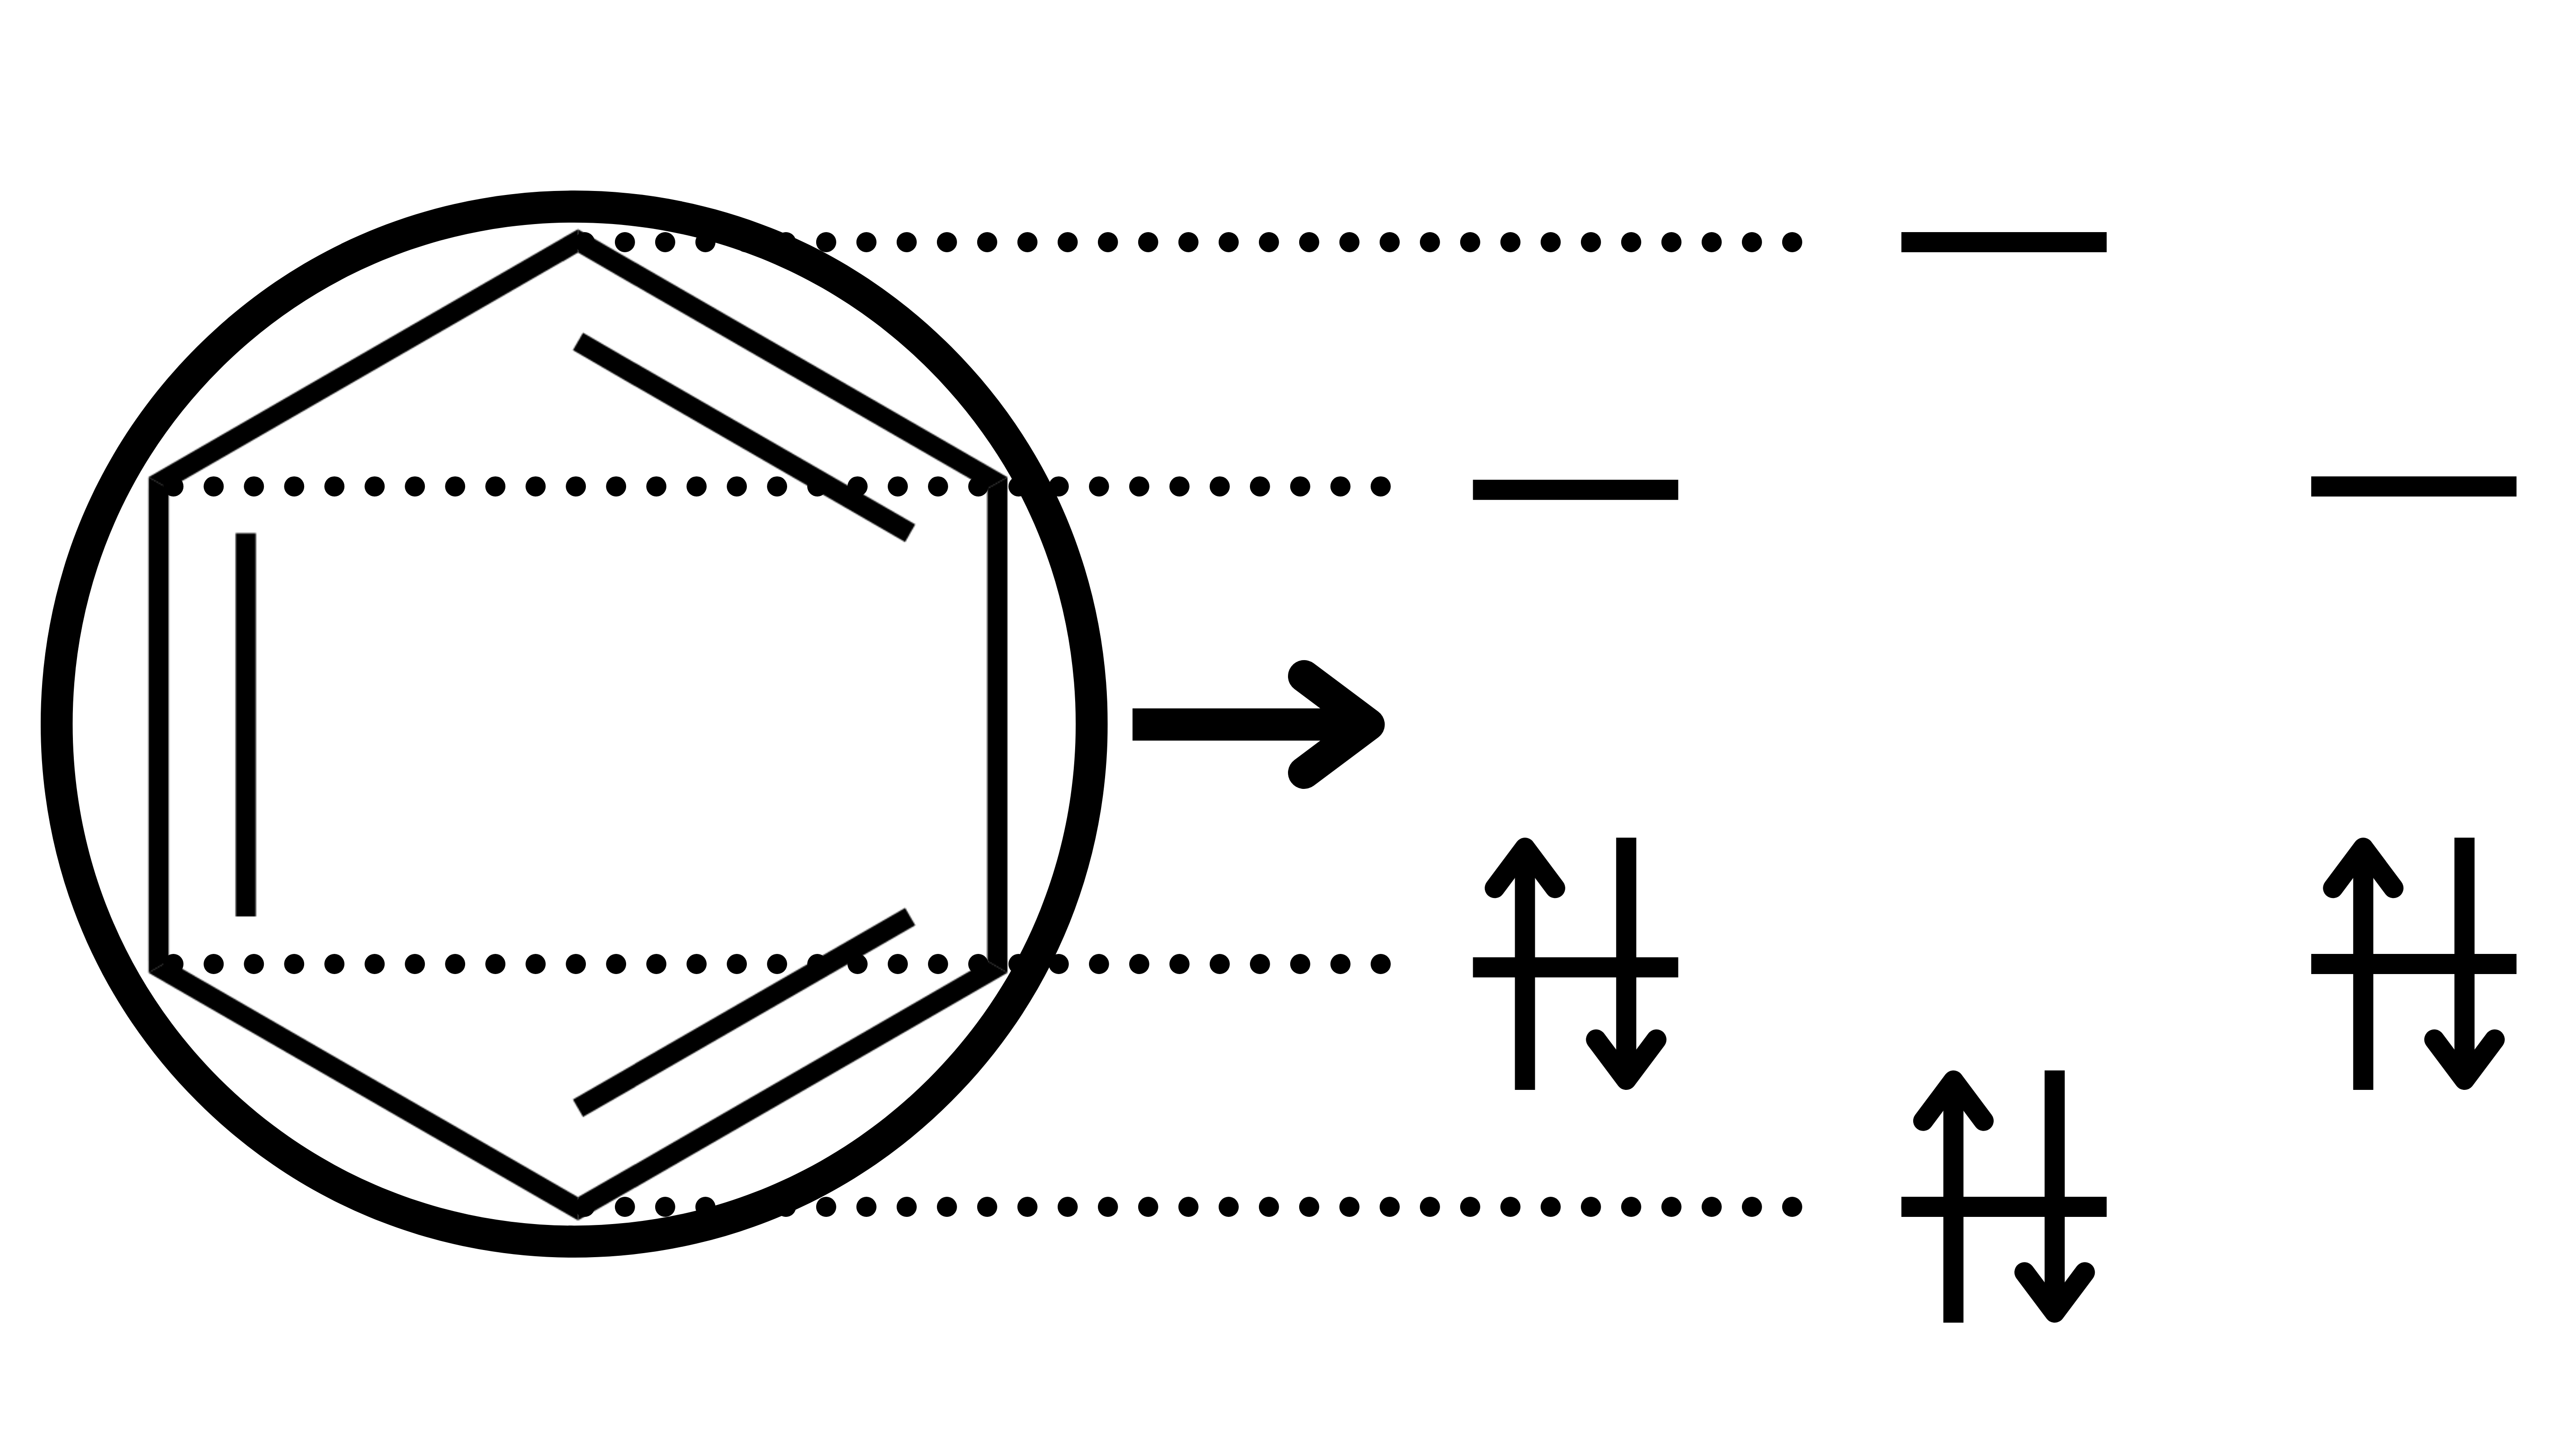
\includegraphics[width=0.70\textwidth]{images/figM.png}
	\end{center}
	\fonte{Autor(a).}
\end{figure}

%%% TODO : FROST DIAGRAM

Posteriormente, essa teoria foi estendida para tratar moléculas com heteroátomos (aqueles diferentes do carbono e hidrogênio)\autocite{Liwschitz1963}. Uma mudança ainda maior foi feita por Roald Hoffmann \autocite{Hoffmann1963}, que desenvolveu o método \gls{EHMO}, o qual inclui todos os elétrons da valência (inclusive elétrons $\sigma$) no cálculo das energias dos orbitais moleculares. Esse método é classificado como semiempírico, ou seja, utiliza dados experimentais para facilitar o processo de cálculo das integrais que acessam a interação elétron-elétron para contabilizar os efeitos de correlação eletrônica na estrutura química.

Como o objetivo do trabalho é desenvolver uma ferramenta rápida e eficiente para ser utilizada dentro no navegador de internet, tal método foi escolhido pelo seu baixo custo computacional de operação, devido às aproximações das matrizes Hamiltonianas pelo teorema de Koopman, responsável por aproximar os valores de $H_{ii}$ pelas energias de ionização

\section{Otimização de geometria}

Predizer o arranjo mais estável dos átomos em uma molécula é uma das mais importantes tarefas na química quântica computacional. Essencialmente, este é um problema de otimização onde a energia total da molécula é minimizada com relação às posições dos núcleos atômicos. A geometria molecular obtida desse cálculo é, dessa forma, um ponto de partida para inúmeras simulações de propriedades moleculares. Se a geometria não é acurada, então quaisquer cálculos que derivam dele também podem ser espúrios.

Uma vez que os núcleos são muito mais pesados do que os elétrons, nós podemos tratá-los como partículas pontuais associadas às suas respectivas posições. A partir disso, é possível afirmar que a energia da molécula $E(x)$.

\section{Teoria de grafos}

\section{Critérios quantitativos da aromaticidade}